\section{灵敏度分析与模型检验}

\subsection{预测模型的时间外检验}

问题一没有使用随机打乱的交叉验证，而是让每个验证窗口严格晚于训练窗口，并在特征重建前把该窗全部观看标签置空。五折扩窗检验的总体结果为 MSE $220.0855$、RMSE $14.8121$、MAE $11.8276$，OOF 残差均值为 $-0.001$ 百万人，说明预测误差在时间外样本上没有明显系统偏移。残差的 $5\%$ 和 $95\%$ 分位数分别为 $-22.7075$ 与 $25.1737$ 百万人，区间两侧大致均衡，但高观看场次仍有一定收缩性低估。因此，预测值适合进入排程模型做相对需求排序，极端场次则应结合经验残差区间保留容量冗余。

为了确认模型选择并非由单一指标偶然决定，我们同时比较 MSE、RMSE 与 MAE。Elastic Net 的三项误差均低于 CatBoost、ExtraTrees 和滚动均值基线，其中相对基线的 RMSE 由 $24.099$ 降至 $14.812$，降幅约 $38.5\%$；相对 CatBoost 的 RMSE 优势为 $0.455$ 百万人，且线性稀疏结构更容易审计赛前字段是否越界。模型选择因此同时满足精度、稳定性和可解释性，而不是只追求训练集上的最低误差。

问题一的另一项检验是把预测输出与后续决策变量解耦。排程优化只接收赛前点预测和经验误差边界，不把实际观看量或赛果重新写回特征表；问题三则在比赛结束后通过独立的状态更新模块改变概率和需求。前后两个时间截面的输入不同但接口清晰，避免了“用赛后事实证明赛前预测准确”的循环论证。

最终模型在五个连续外折上的误差列于表\ref{tab:q1-fold-stability}。训练窗逐步扩展时，RMSE 从 $15.5929$ 总体下降到 $13.2908$，第五折没有因时间距离更远而恶化；第二至第四折虽有波动，但全部低于 $15.5$ 百万人。五折 MSE 的最大值与最小值分别为 $243.1382$ 和 $176.6463$，说明总体均值 $220.0855$ 不是由单个异常折主导。

\begin{table}[htbp]
\centering
\caption{Elastic Net五个时间外折的误差稳定性}
\label{tab:q1-fold-stability}
\begin{tabular}{crrr}
\toprule
外折 & MSE & RMSE & MAE \\
\midrule
1 & 243.1382 & 15.5929 & 12.7572 \\
2 & 226.6187 & 15.0539 & 11.9290 \\
3 & 239.3400 & 15.4706 & 12.2031 \\
4 & 214.6845 & 14.6521 & 11.5100 \\
5 & 176.6463 & 13.2908 & 10.7386 \\
\bottomrule
\end{tabular}
\end{table}

分折结果还提供了部署期监测基准。若新增赛事窗口的 RMSE 超过当前最差折 $15.5929$ 很多，且误差集中在新的赛事类别或时区组合，应优先检查分布漂移和类别编码，而不是直接改变正则化参数；若残差均值显著偏离零，则说明模型出现系统高估或低估，需要重新校准截距或目标尺度。只有当这些诊断在连续窗口复现，才有依据触发完整重训。

验证窗目标历史采用统一口径：每一外折及最早外折的内部调参窗都先屏蔽整段观看标签，再重建目标滞后特征；较早比赛的进球、射门等其他已发生事实仍可滚动进入。该严格口径下 Elastic Net 的 MSE 为 $220.086$，四模型排序与最终 $140+72$ 条预测稳定，说明主结论不依赖验证窗内标签的递推可见性。

\subsection{排程目标权重敏感性}

问题二包含八个经同域归一化的目标分量，基准权重体现价值、观赏性、成本、旅行、公平和风险之间的折中。为检验固定方案对偏好变化的响应，我们在价值权重和风险惩罚权重的二维网格上重新评价已求得赛程；此处只改变评价权重，不重新求解整数规划，因此结果衡量的是“既定方案的评分敏感性”，而不是不同权重下的全局最优前沿。

固定方案在权重网格上的得分变化见图\ref{fig:q2-weight-sensitivity-contour}：取值从 $0.445463$ 变化到 $0.522504$，基准权重比 $(1,1)$ 处为 $0.484946$。价值权重上升时等高线整体向高分方向移动，惩罚权重增加则压低得分；曲面连续且没有局部突跳，说明归一化和符号方向设置一致。

\begin{figure}[htbp]
    \centering
    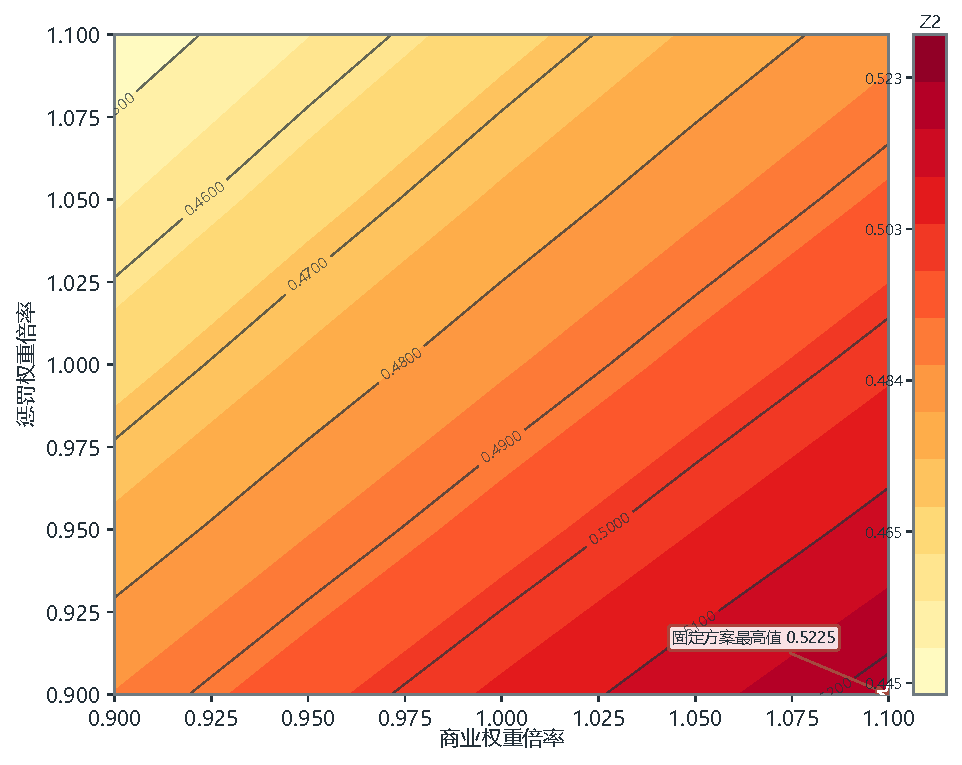
\includegraphics[width=0.85\textwidth,height=0.80\textheight,keepaspectratio]{../figures/fig_q2_weight_sensitivity_contour.pdf}
    \caption{问题二权重敏感性}
    \label{fig:q2-weight-sensitivity-contour}
\end{figure}

最大与最小得分之差为 $0.077041$，约占基准得分的 $15.9\%$，表明综合目标的绝对数值会随偏好改变，但没有出现符号异常或数量级失控。更重要的是，权重变化不改变问题二的硬约束：每队三场、场馆候选、相邻轮休息、日负荷和公平限制仍由同一组布尔变量与约束保证。因而，决策者可在这一曲面上选择偏好点，却不能把权重调整当作放松赛事规则的手段。

求解结果还经过独立的物理复算。$72$ 场均被唯一指派，最小相邻轮休息为 $63$ 小时，场馆负荷为 $2$ 至 $8$ 场，黄金时段次数极差为 $1$，大场馆次数极差为 $1$；全部硬约束无违反。求解器的 incumbent 为 $17811471$、best bound 为 $17883841$，按同一整数目标计算的证书间隙约 $0.41\%$，故应将其表述为满足设定 $0.5\%$ gap limit 的高质量解，而非零间隙证明。

\subsection{动态配置的参数灵敏度}

问题三分别将竞技状态系数和伤病系数乘以 $0.9,1.0,1.1$，形成 $3\times3$ 情景网格。每个情景都保持同一随机数流、共同信息截面、候选动作与日预算约束，并重新计算更新环境和动态最优动作。模型不含“改动惩罚”，因此该检验只衡量状态与伤病反馈参数对目标和资源组合的影响。

该参数网格下的 $Z_3$ 曲面见图\ref{fig:q3-sensitivity-surface}，取值在 $6.623009$ 至 $6.713491$ 之间变化，九个情景的平均晋级概率均为 $2/3$。曲面局部非单调，这是离散动作与日预算共同作用的结果；在所检验范围内没有出现目标数量级突变。

\begin{figure}[htbp]
    \centering
    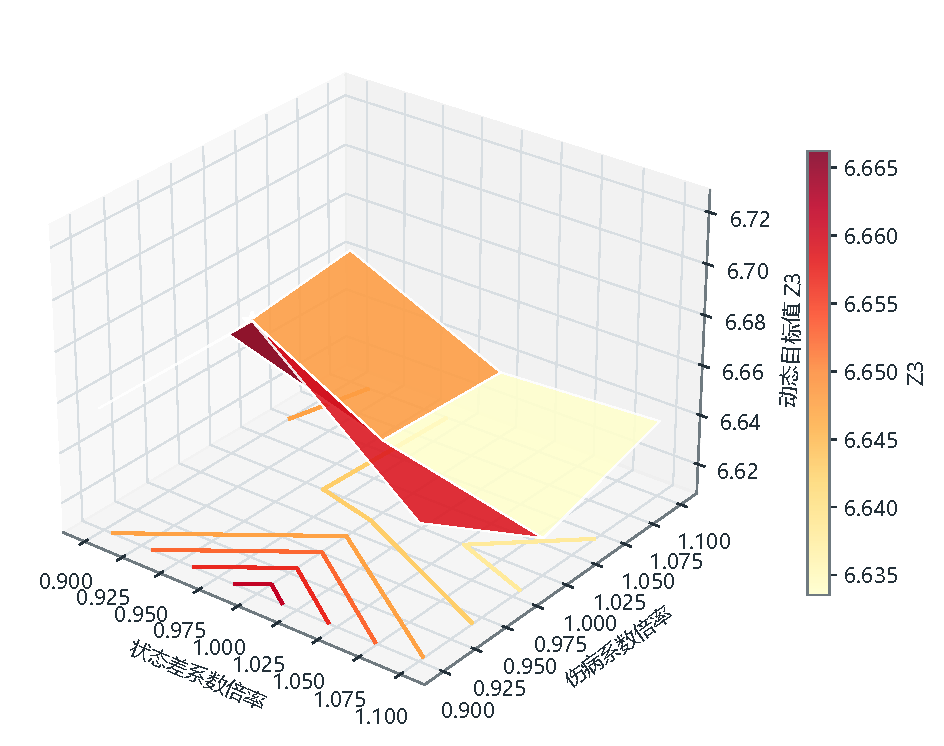
\includegraphics[width=0.85\textwidth,height=0.80\textheight,keepaspectratio]{../figures/fig_q3_sensitivity_surface.pdf}
    \caption{问题三参数敏感性}
    \label{fig:q3-sensitivity-surface}
\end{figure}

九点极差为 $0.090482$，相对中心量级约为 $1.4\%$。这说明动态目标值对所考察的参数扰动较稳定，但稳定并不意味着所有边界场次配置必然不变：基准情景已有 $8$ 场相对静态方案调档。实际执行时仍应把信息更新时间与赛事组织的通知周期共同设定，避免在资源已无法调整后才更新决策。

联合蒙特卡洛自身也经过重复性检验。五个随机种子下晋级概率标准差的最大值为 $0.004691$，且每个种子都重新构造更新环境并完整求解静态与动态资源模型。五次同界增益位于 $[0.065123,0.065434]$，四个附加种子的 $24$ 场动态决策均与基准完全一致，五次求解状态均为 \texttt{OPTIMAL}。因此稳定性不仅体现在边际概率，也落实到最终离散决策。

为避免三维曲面只给出视觉印象，表\ref{tab:q3-sensitivity-grid}列出九个参数点的完整目标值。状态系数倍率从 $0.9$ 增至 $1.1$ 并不保证 $Z_3$ 单调上升，因为动作集合是离散的，参数变化可能使少量边界比赛切换资源档位；伤病系数也通过双方状态、需求和风险共同作用。尽管局部存在非单调，九个点的晋级概率均值都保持 $2/3$，说明名额守恒没有被参数扰动破坏。

\begin{table}[htbp]
\centering
\caption{状态系数与伤病系数扰动下的$Z_3$}
\label{tab:q3-sensitivity-grid}
\begin{tabular}{cccc}
\toprule
状态倍率$\backslash$伤病倍率 & $0.9$ & $1.0$ & $1.1$ \\
\midrule
$0.9$ & 6.657086 & 6.656895 & 6.663519 \\
$1.0$ & 6.713491 & 6.637484 & 6.635101 \\
$1.1$ & 6.661416 & 6.623009 & 6.638511 \\
\bottomrule
\end{tabular}
\end{table}

最大值出现在状态倍率 $1.0$、伤病倍率 $0.9$，最小值出现在 $1.1$、$1.0$。二者并不位于同一参数方向的两个端点，说明目标差异来自离散资源组合与日预算共同形成的分段响应，而不是一个系数符号写反。实际部署若要扩大扰动范围，应在每个新参数点重新求解，不能用当前九点曲面作线性外推。

\subsection{现实比较的权重与代理检验}

问题四的权重扰动和代理扰动给出了不同层次的稳健性结论。在基准最近邻代理下，将八个权重分别上、下调 $10\%$ 后再归一化，共 $16$ 个情景，优化综合得分高于实际方案的方向保持率为 $100\%$。这表明基准方向不是由某个权重的局部微调所决定。

把实际比赛与场馆的全部代理从最近邻整体换成第二近邻后，实际方案得分由 $0.277058$ 变为 $0.226072$，优化方案仍为 $0.480778$，方向没有翻转。完整赛前 Elo、共同包络边界和唯一时段映射保证八项输入均位于 $[0,1]$。代理映射仍是主要不确定性来源，但在已检验邻居范围内不再改变条件性排序。

三种证据状态的对照汇总于表\ref{tab:q4-robustness-levels}。权重扰动下，实际代理分位于 $[0.267908,0.285763]$，优化分位于 $[0.469560,0.491449]$，二者区间不交叠；第二近邻整体替换后仍保持同向。结构层不依赖这些商业和安保邻居，其结论不随该替换改变。

\begin{table}[htbp]
\centering
\caption{问题四不同证据层的稳健性结果}
\label{tab:q4-robustness-levels}
\resizebox{\textwidth}{!}{%
\begin{tabular}{lccc}
\toprule
检验 & 实际赛程 & 优化赛程 & 允许的结论 \\
\midrule
基准最近邻 & 0.277058 & 0.480778 & 优化方向的条件性排序 \\
$16$个权重扰动 & 0.267908--0.285763 & 0.469560--0.491449 & 局部方向稳定 \\
第二近邻整体替换 & 0.226072 & 0.480778 & 邻居方向保持 \\
结构层复算 & 小时、公里、场馆日 & 同单位物理量 & 直接报告事实 \\
\bottomrule
\end{tabular}
}
\end{table}

这一区分说明“方向稳定”必须说明相对于哪一种扰动。权重检验只覆盖决策偏好的局部变化，第二近邻检验只覆盖一个局部代理替换；两者都不能代表真实合同和运营成本。现实 $48$ 场仍只映射到 $26$ 个题内比赛和 $4$ 个题内场馆，最高复用次数分别为 $6$ 和 $33$。只有结构层的来源与公式都能从逐场记录复核，因此其证据强度仍高于两个代理得分情景。

综合四问的检验结果可见，预测误差、权重偏好、状态反馈和代理映射属于四种不同的不确定性。前两类主要改变数值幅度，硬约束仍保持；第三类决定少量场次是否需要动态调档；第四类在已检验范围内未改变方向，却仍限制结论能否外推到真实运营。分层报告这些影响，比把所有扰动混合成一个“鲁棒性分数”更能说明模型的适用边界。
